\begin{chapter}{Implementacja głównej aplikacji WikiGraph}
	\newcommand{\chapterPath}{rozdzialy/4_implementacja}

	\section{Model danych}
Model danych aplikacji tworzony jest na podstawie plików opisanych w \ref{sec:data-files}. Są one otwierane jako strumienie używając klasy \lstinline[basicstyle=\normalsize]{FileStream} co pozwala na jednakowy dostęp do każdej części pliku. 

Listing \ref{lst:node-model} zawiera używany przez aplikację model węzła. Przy żądaniu załadowania do pamięci węzła o konkretnym numerze (\ref{line:nm-id}) najpierw odczytywane są informacje z pliku mapy a następnie na ich podstawie wczytywany jest tytuł (\ref{line:nm-title}) oraz połączenia węzła (\ref{line:nm-children} i \ref{line:nm-parents}). Określany jest też typ węzła (\ref{line:nm-type}) oraz jego identyfikator przypisany przez Wikipedię (\ref{line:nm-wikiid}). Na koniec nowo wczytanemu węzłowi zostaje przypisany stan (\ref{line:nm-state}) aktywny.
\begin{lstlisting}[caption={Model węzła grafu}, label=lst:node-model]
public class Node {
	public uint[] Children; %*\label{line:nm-children}*)
	public uint[] Parents; %*\label{line:nm-parents}*)

	public readonly uint ID; %*\label{line:nm-id}*)
	public uint WikiID; %*\label{line:nm-wikiid}*)

	public string Title; %*\label{line:nm-title}*)

	public NodeType Type; %*\label{line:nm-type}*)
	public NodeState State; %*\label{line:nm-state}*)
	%*\dots*)
}
\end{lstlisting}

Załadowane węzły są dodawane jako wartości w mapie ID $\,\to\,$ \codeinline{Node} co pozwala na późniejsze szybkie uzyskanie modelu na podstawie jego identyfikatora. Przechowywanie grafu w pamięci zostanie szczegółowo opisane w \ref{sec:graf-reprezentacja}.

W wyniku interakcji użytkownika z węzłem pokazywane są połączenia, Zostały one zamodelowane jako zbiór dwóch węzłów. Przy tym przyjmujemy że połączenie zaczyna się w węźle z którym nastąpiła interakcja.

	\section{Wizualna reprezentacja grafu}
\sectionauthor{Stanisław Góra}
\label{sec:graf-reprezentacja}

\newcommand\mapitem[3]{
	\item \textbf{#1 $\to$ #2}

	#3
}

% Przechowywanie grafu w pamięci
\noindent
Graf jest przechowywany w pamięci aplikacji jako zbiór map:
\begin{enumerate}[label=\textbullet]
	\mapitem{Identyfikator węzła}{Model węzła}{Opisana już mapa warstwy modelu}
	\mapitem{Model węzła}{Obiekt wizualny węzła}{Przechowuje widoczne aktualnie w aplikacji węzły jako wartości przypisane do modelu reprezentowanego węzła. Obiekt wizualny przechowuje numer ID węzła, co zamyka pętlę powiązań, i w efekcie pozwala na uzyskanie informacji o węźle (z jego modelu), mając na wejściu jego obiekt wizualny na podstawie dwóch map.}
	\mapitem{Model połączenia}{Obiekt wizualny połączenia}{Mapa analogiczna do poprzedniej, przechowująca informacje o połączeniach między węzłami. Podobnie obiekt wizualny połączenia przechowuje dwa identyfikatory węzłów które łączy.}
	
	\mapitem{Model połączenia}{Obiekt wizualny reprezentacji węzła końcowego połączenia}{Mapa przechowująca pomocnicze reprezentacje węzłów końcowych połączenia opisane szczegółowo w sekcji \ref{sec:tryby-widoki}.}
\end{enumerate}

% GO Node - Billboard Shader
\subsection{Reprezentacja węzła} Z uwagi na dużą ilość jednocześnie załadowanych węzłów (kilka do kilkunastu tysięcy na raz) konieczne okazały się pewne optymalizacje, poprawiające szybkość działania aplikacji. 

Obiekty węzłów nie są w większości przypadków tworzone dynamicznie. Zamiast tego przy starcie aplikacji tworzona jest pula nieużywanych obiektów. W momencie ładowania węzła nowy obiekt wizualny tworzony jest tylko w przypadku, kiedy pula została wyczerpana. Przy usuwaniu węzła jego reprezentacja nie jest niszczona, tylko zwracana do puli w celu przyszłego wykorzystania.

W celu odciążenia karty graficznej zrezygnowaliśmy z wyświetlania każdego węzła jako trójwymiarowego modelu (jak na przykład kuli). Reprezentacją węzła jest prosta grafika rastrowa (Rysunek \ref{fig:node_sprites}). Jest ona dużo szybsza do przetworzenia, ponieważ zawiera tylko cztery wierzchołki - jest to kwadratowa płaszczyzna z nałożoną teksturą. Dzięki temu aplikacja jest w stanie wyświetlić więcej węzłów na raz bez utraty płynności działania.

\img{\chapterPath/img/node_sprites.png}{Grafiki węzłów (od lewej): artykuł aktywny i wskazany, kategoria aktywna i wskazana}{node_sprites}{0.6}

Takie rozwiązanie powoduje jednak pewną komplikację. Płaszczyzna z grafiką, w przeciwieństwie do przestrzennego modelu, jest dobrze widoczna tylko kiedy kamera jest ustawiona bezpośrednio przed nią. Pojawia się więc potrzeba obracania obiektu węzła tak, aby był on zawsze zwrócony przodem do użytkownika zwiedzającego graf. Najprostszym rozwiązaniem byłoby dodanie krótkiego skryptu do każdego obiektu, który przy każdym odświeżeniu ekranu obracałby reprezentację węzła w stronę kamery. Nie jest to jednak dobre rozwiązanie z powodu narzutu czasowego. W każdej klatce ta sama operacja byłaby wykonywana potencjalnie kilkanaście tysięcy razy, co mogłoby mieć widoczny efekt na szybkości działania.

Poprawnym rozwiązaniem jest użycie shadera. W przeciwieństwie do standardowych skryptów aplikacji jego działanie jest zrównoleglone przez kartę graficzną dla potencjalnie każdego przetwarzanego wierzchołka. Tu jednak natrafiliśmy na kolejny problem. Powszechnie stosowane są tak zwane ``Billboard Shadery'', które służą dokładnie do interesującego nas celu, jednak w szczególnym przypadku aplikacji budowanej na środowisko LZWP są niewystarczające. Każda ściana jaskini jest kontrolowana przez osobny komputer z osobną instancją aplikacji, posiadającą osobną kamerę skierowaną w kierunku danej ściany. Billboard Shader odwraca obiekty węzłów w kierunku kamery na lokalnej ścianie, co powoduje, że jeśli dany obiekt znajdzie się w pozycji wyświetlanej na przecięciu ekranów (połowa węzła na jednej a połowa na drugiej ścianie jaskini), na każdym z odpowiadających za ściany komputerów zostanie obrócony w lekko innym kierunku. W efekcie części obiektu węzła mogą nie być spójne.

Aby rozwiązać ten problem, należało wybrać obiekt wspólny dla wszystkich ścian, a następnie obracać grafiki węzłów w względem niego zamiast kamer. To wymagało ręcznego przepisania shadera z powodu braku gotowego i dostępnego rozwiązania. Problem sprowadził się do stworzenia macierzy \(R\) przekształcającej wektor trójwymiarowy \(a\) w \(b\) - w tym przypadku domyślny zwrot grafiki węzła w kierunek wybranego obiektu wspólnego. Implementacja jest wzorowana na wpisie z forum matematycznego \cite{BillboardShaderFormula}.

\newcommand\dotProd{a \cdot b}
\newcommand\crossProd[1]{(\overrightarrow{a \times b})_#1}
\begin{equation}
	R = I + [v]_{\times} + [v]_{\times}^2\frac{1}{1 + c}
\end{equation}
\begin{equation}
	[v]_{\times} \stackrel{\rm def}{=} 
	\begin{bmatrix}
		0 & -v_z & v_y\\
		v_z & 0 & -v_x\\
		-v_y & v_x & 0
	\end{bmatrix}
\end{equation}
,gdzie:
\begin{itemize}
	\item \(v = a \times b\)
	\item \(c = a \cdot b\)
\end{itemize}

% GO Connection - B-Spline
\subsection{Reprezentacja połączenia}
Połączenia są w aplikacji reprezentowane jako krzywe (Rysunek \ref{fig:node-connections}). Ich kształt został najpierw zawinięty w górę tak, aby przechodzić przez stworzone dla każdego połączenia węzły pomocnicze opisane w sekcji \ref{sec:tryby-widoki}, a następnie zmierza łukiem w kierunku faktycznego węzła końcowego. Na początku do tworzenia tras połączeń używane były krzywe Béziera, jednak obecnie, z powodu ich skomplikowanego kształtu, zastąpione zostały krzywymi B-Spline zaimplementowanymi według algorytmu De Boor'a.

\img{\chapterPath/img/connections.png}{Wygląd węzłów i połączeń w aplikacji}{node-connections}{.9}

	\section{Tryby poruszania się i widoki węzła}
\sectionauthor{Mikołaj Mirko}
\label{sec:tryby-widoki}
Aplikacja posiada dwa tryby poruszania się: swobodne latanie oraz podróżowanie po węzłach. Pierwszy z nich charakteryzuje się pełną swobodą przemieszczania się. Po wskazaniu kierunku kontrolerem i pochyleniu joysticka do przodu, kamera zaczyna przemieszczać się do przodu, przy odchyleniu joysticka do tyłu w przeciwną stronę. Otaczająca użytkownika przestrzeń jest wizualnie wzorowana na przestrzeni kosmicznej (skybox posiada przygotowaną teksturę imitującą gwiaździste niebo). Rozmieszczone w tej przestrzeni węzły (artykuły i kategorie) można wskazywać i wybierać. W przypadku wskazania jednego z nich wyświetlany jest podgląd jego pierwszych połączeń (jeżeli jakiekolwiek posiada). Rysunek \ref{fig:widok_grafu} prezentuje ten scenariusz na przykładzie artykułu ``Gdańsk''.

\img{\chapterPath/img/widok_grafu.png}{Widok grafu ze wskazanym węzłem i podglądem jego połączeń}{widok_grafu}{.9}

Po wybraniu węzła (naciśnięciu przycisku spustu na kontrolerze) użytkownik umieszczany jest w~widoku węzła i~wykorzystuje tryb poruszania się po węzłach. W tym momencie kamera umieszczana jest nad wybranym węzłem, a linie połączeń wypełniają się kolorem. Nieaktywne węzły są wygaszane, aby~zwiększyć przejrzystość widoku węzła. W każdej chwili można powrócić do widoku grafu i swobodnego latania klikając przycisk oznaczony jako \textit{Exit} na kontrolerze. Na rysunku \ref{fig:widok_wezla} znajduje się przykładowy wygląd wychodzących połączeń z artykułu ``Politechnika Gdańska'' ze wskazanym artykułem ``Technologia'' i podglądem jego połączeń. Przemieszczanie w tym trybie polega głównie na~przechodzeniu z węzła na węzeł poprzez dostępne połączenia. Cofanie się po przebytej drodze to inny sposób trawersowania w tym trybie – został on szczegółowo opisany w sekcji \ref{sec:history}.

\img{\chapterPath/img/widok_wezla.png}{Widok węzła z połączeniami i zaznaczonym powiązanym węzłem}{widok_wezla}{.9}

Widok węzła składa się z dwóch części. Pierwsza z nich definiuje wyświetlane połączenia jako wychodzące z wybranego węzła (jest to domyślne rozwiązanie). Drugą częścią są połączenia, które docierają z innych węzłów do aktualnie wybranego. Aby przełączyć się między widokami, należy nacisnąć spust wskazując kontrolerem w aktualnie wybrany element, znajdujący się na dolnym ekranie. Różnice pomiędzy tymi rodzajami połączeń (oraz sposoby ich pozyskiwania) zostały opisane w sekcji \ref{sec:generating-missing-files}.
	\section{Elementy zwiększające użyteczność aplikacji}
\sectionauthor{Mikołaj Mirko}
\label{sec:elementy}
Jednym z ważniejszych elementów znajdujących się w aplikacji jest podążający za wzrokiem nagłówek z informacjami o stanie grafu. Umiejscowiony jest on powyżej linii wzroku tak, aby nie przeszkadzał w interakcji z węzłami, a zarazem był wyraźnie widoczny z każdego miejsca oraz kąta patrzenia. Jego pozycja pionowa jest zaczepiona w stałym punkcie, a pozycja pozioma uzależniona od kierunku wyznaczanego przez główne okulary jaskini.

Na samej górze znajduje się informacja o tym, czy węzeł jest tylko wskazywany kontrolerem, czy jesteśmy w widoku grafu z aktualnie wybranym węzłem. Zaraz pod spodem widoczny jest tytuł artykułu lub kategorii. W trybie swobodnego latania nagłówek wyświetlany jest tylko w przypadku wskazywania węzłów. Rysunek \ref{fig:header1} nakreśla układ nagłówka po wskazaniu artykułu ``Matematyka''. Jeśli węzeł posiada jakieś połączenia, ich liczba wyświetlana jest pod tytułem.

\img{\chapterPath/img/header1.png}{Nagłówek po wskazaniu węzła}{header1}{.8}

Dla widoku węzła dostępna jest większa ilość informacji. Pod tytułem pojawia się podłużny wskaźnik przypominający poziomy pasek przewijania. Wraz z informacją tekstową, znajdującą się tuż pod nim, określa aktualnie wyświetlany wycinek listy połączeń. Łatwo zauważyć, które połączenia są wyświetlane wokół użytkownika oraz jaką część stanowią. Na Rysunku \ref{fig:header2} wybrany został artykuł zatytułowany ``Wstęga Möbiusa'' z 21 połączeniami wychodzącymi (aktualnie wyświetlane są połączenia od pierwszego do ósmego włącznie).

\img{\chapterPath/img/header2.png}{Nagłówek w widoku węzła z informacją o połączeniach}{header2}{.8}

Ostatnią częścią nagłówka jest ikona stanu. Zawiera ona 3 istotne informacje: rodzaj węzła (artykuł lub kategoria), aktualny typ połączeń (wychodzące z węzła lub do niego trafiające) oraz wariant poruszania się. Rodzaj węzła jest ilustrowany poprzez kolor oraz kształt (Rysunek \ref{fig:node_sprites}). O typie połączeń świadczy również kolor, a także skierowanie strzałek w stosunku do symbolu węzła. (Na Rysunku \ref{fig:header2} ikona oznacza artykuł z połączeniami wychodzącymi). Domyślnym wariantem poruszania się jest ręczne przeskakiwanie z węzła na węzeł. Przy uruchomionej zaprogramowanej trasie (czyli automatycznym przechodzeniu po zdefiniowanej ścieżce - więcej o tym w sekcji \ref{sec:history}) na symbolu węzła pojawia się fraza \textit{AUTO} (Rysunek \ref{fig:header3}).

\img{\chapterPath/img/header3.png}{Nagłówek z ikoną stanu sygnalizującą trwające automatyczne przemierzanie trasy}{header3}{.8}

Aplikacja została dodatkowo wyposażona w elementy wspomagające pracę z grafem. Na dolnym ekranie widoczne są półprzezroczyste linie pomocnicze określające płaszczyznę podłoża. Przemieszczają się one z kamerą i mają na celu zapewnienie punktu odniesienia do innych obiektów otaczających użytkownika. Opisana siatka widoczna jest na Rysunku \ref{fig:widok_wezla}.

Kolejnym elementem jest przestrzeń pomocy. Jest to specjalna przestrzeń wydzielona od struktury grafu, do której można wejść w dowolnej chwili korzystania z aplikacji. Użytkownik jest w niej umieszczany również na starcie programu. Zawiera ona podstawowe informacje o programie, a także zestaw infografik zapoznających użytkownika ze sposobami sterowania i możliwościami aplikacji (Rysunek \ref{fig:info_space}).

\img{\chapterPath/img/info_space.png}{Jedna z infografik dostępnych w przestrzeni pomocy}{info_space}{.8}

Dodatkowo na potrzeby aplikacji została stworzona muzyka. Przez cały czas działania aplikacji w tle odtwarzany jest klimatyczna ścieżka dźwiękowa w gatunku ambient wzmacniająca immersję. Ponadto każda akcja użytkownika ma przypisany inny efekt. Sygnalizuje on użytkownikowi, że aplikacja poprawnie odebrała wciśnięcie przycisku, co zwiększa intuicyjność sterowania. Co więcej, sygnalizuje specjalne akcje takie jak zmiana trybu przeglądania, czy włączenie lub wyłączenie pomocy.
	\section{Historia przeglądania oraz zaprogramowane trasy}
Specyfika działania aplikacji, związana z wykonywaniem przez użytkownika akcji nawigacyjnych, oraz środowisko działania skłoniły do zaimplementowania funkcjonalności związanych z historią. Znacząco ułatwią i przyspieszą one poruszanie się po węzłach grafu. Bez możliwości skorzystania z historii użytkownik byłby zmuszony do każdorazowego szukania poprzedniego węzła  w grafie bądź w odpowiednim widoku wybranego węzła. Co więcej, aby zapewnić powtarzalność podczas prezentacji, a także, aby wyeksponować ciekawe przypadki połączeń pomiędzy węzłami, będzie możliwe zapisanie tras przeglądania. Odtwarzanie tras umożliwia dokładne planowanie prezentacji i eliminuje problemy wynikające z losowości wyświetlania węzłów. 

Do historii zapisywane są tylko akcje kluczowe dla nawigacji - zmiana widoku wyświetlania oraz wybieranie węzłów. Inne działania użytkownika nie powodują znaczących zmian w nawigacji po grafie i ich przechowywanie jest bezcelowe. Po naciśnięciu Przycisku 2 na kontrolerze wywoływana jest poprzednia akcja wykonana przez użytkownika. Odpowiednio, aby ponowić cofniętą akcję, należy nacisnąć Przycisk 3. W przypadku braku akcji do ponowienia lub cofnięcia nie jest podejmowane żadne działanie. Wywoływanie i zapisywanie tras dostępne jest z poziomu konsoli operatora opisanej w następnym punkcie.


Akcje użytkownika są przechowywane jako odpowiednie klasy dziedziczące po klasie UserAction. Posiada ona wirtualne funkcje Execute() oraz UnExecute() służące odpowiednio ponawianiu i cofaniu akcji. Każda akcja posiada także swojego własnego delegata, zależnego od typu akcji. 

Bezpośrednie operacje na historii wykonywane są przez HistoryService. Przechowuje on akcje użytkownika we dwu stosach: pierwszy służy zapisywaniu akcji do cofnięcia, drugi akcji do ponowienia. W momencie wciśnięcia przycisku 2 wyzwalane jest zdarzenie wywołujące funkcję UndoAction(), która poza wykonaniem kolejnego zdarzenia wywołującego funkcję akcji odpowiedzialnej za cofanie, zdejmuje tę akcję ze stosu akcji do cofania i wkłada na stos akcji do ponawiania.

Wszystkie delegowane funkcje służące historii oraz trasom są przypisywane w kontrolerze HistoryController. Warunkiem jest, aby aplikacja była serwerem.

Zaznaczanie węzłów z historii oraz zmiana widoku odbywa się w identyczny sposób, jak zwykłe wywoływanie tych akcji przy użyciu kontrolera, jednak nie są one ponowne zapisywane do historii, jak przy zwykłym wywołaniu.

Analogicznie do modułu historii zaprojektowane zostało odtwarzanie tras. Pliki zawierające trasy posiadają rozszerzenie .wgroute. Struktura pliku jest stosunkowo prosta - pierwsza cyfra służy rozróżnieniu akcji użytkownika: 0 oznacza zmianę widoku, a 1 wybranie węzła. W przypadku zmiany widoku po średniku można znaleźć cyfrę 0 lub 1. 0 odpowiada zmianie widoku na na widok dzieci, a 1 zmianie widoku na widok rodziców. Jeśli akcją było wybranie węzła, po średniku znajduje się ID artykułu do wybrania. 

Po wybraniu trasy rozpoczyna się proces jej wczytywania. Są za to odpowiedzialne dwie klasy: RoutesReader oraz RoutesLoader. Pierwsza ma za zadanie pobrać dostępne trasy, ich nazwy i długość oraz wczytywać kolejne linijki plików. Druga przekształca wczytane dane linijka po linijce na odpowiednie akcje i dopisuje do stosu.

W momencie włączenia trasy inicjowane jest wczytanie trasy z plików, a po tej operacji tworzony jest współprogram(ang. coroutine), która ma za zadanie wykonywanie kolejnych akcji trasy co daną liczbę sekund. Odtwarzanie trasy sygnalizowane jest przez ikonę AUTO w nagłówku. W każdym momencie możliwe jest wyłączenie odtwarzania trasy za pomocą Przycisku 4, powodującego zatrzymanie współprogramu. W przypadku włączenia innej trasy w trakcie odtwarzania, współprogram poprzedniej trasy jest także wyłączany, a następnie wczytywana i inicjalizowana jest nowa trasa. 

	\section{Integracja z jaskinią rzeczywistości wirtualnej}
\sectionauthor{Stanisław Góra}
Laboratorium Zanurzonej Wizualizacji Przestrzennej \cite{LZWP_article} posiada szereg innowacyjnych rozwiązań z zakresu rzeczywistości wirtualnej. Największą instalacją jest wykorzystywana w tym projekcie duża jaskinia będąca sześciennym pomieszczeniem o boku 3,4m. Na każdą ze ścian wyświetlany jest z zewnątrz obraz z dwóch projektorów zdolnych stworzyć projekcję stereoskopową odbieraną przy pomocy okularów migawkowych \cite{IntegraAV}. Sterowanie symulacją odbywa się poprzez użycie kontrolera z joystickiem oraz pięcioma przyciskami. Dodatkowo zainstalowany jest system śledzenia ruchu pozwalający na wykrycie położenia kontrolera oraz okularów osoby sterującej symulacją.

% LZWPLib
Przystosowanie aplikacji do działania w środowisku LZWP dzieli się na dwa podzadania: obsługa wejścia użytkownika oraz synchronizacja stanu aplikacji pomiędzy komputerami obsługującymi ściany jaskini. Reszta integracji jest zapewniana przez stworzoną przez pracowników LZWP bibliotekę.

% Input Module
\subsection{Moduł wejścia}
W założeniu aplikacja ma wspierać dwie metody interakcji użytkownika, nazywane później środowiskami:
\begin{enumerate}[label=\textbullet]
	\item \textbf{PC} - gdzie użytkownik posługuje się klawiaturą i myszą, używane głównie podczas procesu wytwarzania aplikacji
	\item \textbf{Jaskini} - gdzie użytkownik nosi okulary i trzyma specjalny kontroler nazywany flystickiem
\end{enumerate}
Aby ułatwić sobie wytwarzanie głównej logiki aplikacji, wejście zostało odseparowane w osobny moduł, który może być przed uruchomieniem ustawiony w jeden z dwóch trybów, odpowiadającym każdemu środowisku. Tryb ten definiuje jakiego rodzaju wejścia ma nasłuchiwać aplikacja. Moduł wejścia składa się z trzech mniejszych części:
\paragraph{Definicje akcji użytkownika}
Ustala wspólny interfejs dla każdej akcji użytkownika dostępnej w aplikacji. Są to między innymi: 
\begin{enumerate}[label=\textbullet]
	\item Użycie przycisku klawiatury i myszy (PC) lub flysticka (jaskinia)
	\item Przesunięcie myszy (PC) lub flysticka (jaskinia)
\end{enumerate}
Oprócz tego jest odpowiedzialna za nasłuchiwanie wykonania przez użytkownika swojej akcji i odpowiednie powiadomienie aplikacji.

\paragraph{Definicje akcji aplikacji}
Spis akcji wykonywanych w aplikacji. Są to między innymi: 
\begin{enumerate}[label=\textbullet]
	\item Wybranie lub podświetlenie węzła
	\item Poruszanie się po grafie
	\item Zmiana zakresu wyświetlanych połączeń
\end{enumerate}
Każda akcja ma swój typ (opisany w poprzednim punkcie). Dostępny jest też interfejs, dzięki któremu możliwe jest łatwe wybranie konkretnego przycisku (w każdym ze środowisk), który ma aktywować daną akcję (rysunek \ref{fig:input-interface}).

\paragraph{Procesor akcji użytkownika}
Odpowiada za połączenie modułu wejścia z pozostałą częścią aplikacji poprzez powiadamianie jej o każdej wykonanej przez użytkownika akcji po ewentualnym wstępnym przetworzeniu sygnału wejściowego.


\img{\chapterPath/img/input-interface.png}{Fragment interfejsu wyboru przycisków dla środowiska PC}{input-interface}{.6}

% Networking
\subsection{Synchronizacja stanu}
Jak już zostało wspomniane, w LZWP każda ściana jaskini sterowana jest przez osobny komputer. Oznacza to, że środowisko aplikacji podobne jest do wieloosobowej gry w sieci LAN i wymusza synchronizację stanu z głównym komputerem, odpowiedzialnym za przetwarzanie akcji użytkownika. W tym celu powstał w aplikacji moduł wysyłający zmiany w grafie komputerom do aktualizacji ekranów. Cały proces zaprezentowany został na diagramie na rysunku \ref{fig:diagram-modolow}.

Na opisanie zasługuje tu synchronizacja załadowanych lub usuniętych węzłów grafu. Mechanizm przesyłający wiadomości w sieci jest dosyć prosty i pozwala na dołączanie tylko najprostszych typów danych jak ciąg znaków, liczby i pozycja. Wysyłanie informacji o załadowaniu każdego węzła z osobna mogłoby zapełnić kanał komunikacyjny zwłaszcza przy starcie aplikacji, kiedy ładowane są tysiące węzłów na raz. Został więc wprowadzony mechanizm, którego celem jest zbieranie tych komunikatów i łączenie ich w większe paczki, które po przesłaniu są z powrotem rozpakowywane i przetwarzane. Dzięki temu aplikacja zachowuje optymalne wykorzystanie łącza w jaskini.

\begin{figure}[H]
\begin{center}
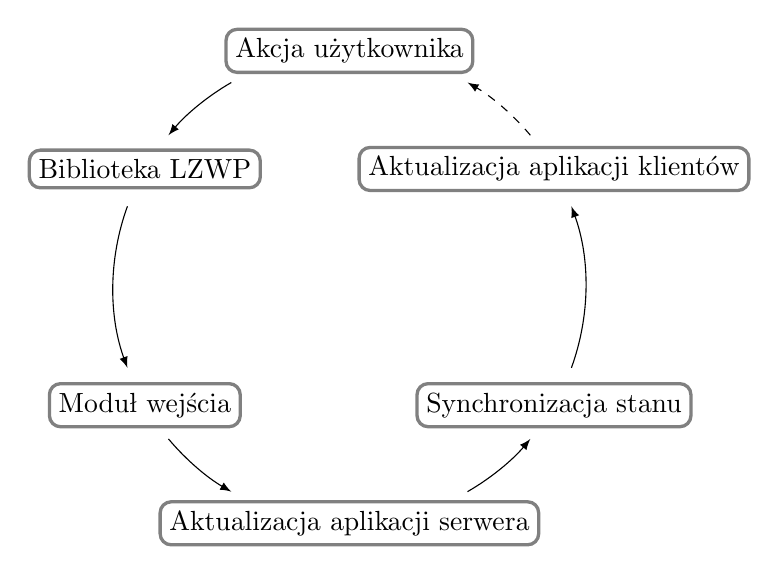
\begin{tikzpicture}[stepstyle/.style={rectangle, 
		rounded corners, draw=gray, very thick,
		text centered, align=center}]
	\def \n {6}
	\def \offset {30}
	\def \radius {3cm}

	\foreach \step [count=\s] in {Akcja użytkownika, Biblioteka LZWP, Moduł wejścia, Aktualizacja aplikacji serwera, Synchronizacja stanu, Aktualizacja aplikacji klientów} {
		\node(\s) [stepstyle] at ({360/\n * (\s) + \offset}:\radius) {\step};
	};
	\foreach \b/\e in {120/140, 160/200, 220/240, 300/320, 340/380} {
		\draw[->, >=latex] ({\b}:\radius)
		arc ({\b}:{\e}:\radius);
	};
		\draw[dashed, ->, >=latex] ({40}:\radius)
		arc ({40}:{60}:\radius);
\end{tikzpicture}
\end{center}
\caption{Diagram kolejności wykonywania modułów przy akcji użytkownika}
\label{fig:diagram-modolow}
\end{figure}



	\section{Konsola operatora}

	\section{Linia czasu}
\sectionauthor{Mateusz Janicki}
\label{sec:linia-czasu}
Specyfikacja wymagań projektu inżynierskiego zawierała funkcjonalność dotyczącą linii czasu. Wybranie daty miało spowodować wyświetlanie tylko takich węzłów, których data utworzenia była starsza niż wybrana data. Pomogłoby to w przybliżonej wizualizacji, w jak szybki sposób rozrastała się konkretna Wikipedia. Szereg komplikacji spowodował jednak odrzucenie przez nas tej funkcjonalności.

Sterowanie linią czasu miało odbywać się za pomocą drugiego kontrolera. Po wciśnięciu przycisku miał pokazywać się specjalny interfejs ukazujący aktualnie wybraną datę. Można w niej było wybrać, przesuwając joystick w lewo i prawo, miesiąc lub rok, który następnie dałoby się zmieniać przesuwając joystick do góry lub w dół. Zatwierdzenie daty przyciskiem spustu wywoływałoby zmiany w grafie. 

Funkcjonalność nie została zaimplementowana głównie z powodu braku prostej informacji o stworzeniu artykułu w głównie wykorzystywanym przez nas źródle danych, czyli zrzutach baz danych Wikipedii. Istnieją archiwa zawierające kompletną historię edycji artykułów, jednak wielkość tych plików jest nieporównywalnie większa w porównaniu ze zwykłym wykazem stron czy nawet połączeniami pomiędzy stronami. Przetworzenie tych plików tylko po to, aby wydobyć z nich datę pierwszej publikacji strony, jest niewymierna do korzyści wynikających z tej funkcjonalności. 

Innym sposobem wydobycia danych mogłoby być pozyskiwanie tych informacji przy użyciu Wikipedia API. Pomysł ten jednak nie jest wykonalny z powodu ograniczeń, które posiada API. Aby~zdobyć informacje dotyczące każdego artykułu, musielibyśmy wywołać zapytania, których liczba znacznie przewyższa maksymalną dopuszczalną liczbę zapytań dla jednego użytkownika. Przekroczenie tej liczby powoduje zablokowanie adresu IP, z którego pochodziły zapytania i utrudnia dalsze pozyskiwanie danych.

Co więcej, nasza idea linii czasu nie byłaby dokładnym odwzorowaniem stanu Wikipedii w wybranym przez użytkownika czasie. Artykuły i kategorie Wikipedii są bardzo często zmieniane, co implikuje możliwość zmiany połączeń pomiędzy artykułami. Ponadto artykuły i kategorie mogą być także usuwane. Przechowywanie całej historii stron lub stworzenie plików zawierających dokładną historię wszystkich węzłów, jakie kiedykolwiek pojawiły się w Wikipedii, jest niemożliwe na zwykłych komputerach osobistych z powodu zbyt dużej wymaganej przestrzeni na dysku. Nawet jeśli udałoby się je~zapisać, przetwarzanie i wczytywanie takich plików zajęłoby bardzo dużo czasu i spowodowałoby niską responsywność aplikacji. Nasza wersja linii czasu mogłaby być myląca dla nowych użytkowników, którzy mogliby pomyśleć, że przedstawiana jest im dokładna wersja Wikipedii w danym czasie.
\end{chapter}



